% !TeX program = lualatex

\documentclass[12pt]{article}



\usepackage[margin=1in]{geometry} 
\usepackage{amsmath,amsthm,amssymb}
\usepackage{MnSymbol}
\usepackage{graphicx}
\usepackage{bm}
\usepackage[normalem,normalbf]{ulem}
\usepackage{algorithm} 
\usepackage{algpseudocode} 
\usepackage{multirow}
\usepackage{rotating}
\usepackage{therefore}

\usepackage{tikz}
\usetikzlibrary{shapes.multipart}
\usetikzlibrary{shapes.symbols}

\usetikzlibrary{graphs,graphdrawing,graphs.standard,quotes}
\usegdlibrary{circular,force,layered,routing}
\tikzset{
	graphs/simpleer/.style={
		nodes={draw,circle, blue, left color=blue!20, text=black, inner sep=1pt},
		node distance=2.5cm, nodes={minimum size=2em}
	},
	every loop/.style={},
}

\newcommand*\circled[1]{\tikz[baseline=(char.base)]{
		\node[shape=circle,draw,inner sep=2pt] (char) {#1};}}

\newcommand{\m}{\medskip\\}
\newcommand{\N}{\mathbb{N}}
\newcommand{\Z}{\mathbb{Z}}
\newcommand{\R}{\mathbb{R}}
\newcommand{\bbs}{\textbackslash\textbackslash\space}
\newcommand{\bs}{\textbackslash\space}
\newcommand{\la}{\enskip\land\enskip}
\newcommand{\lo}{\enskip\lor\enskip}
\newcommand{\comp}[1]{#1^\mathsf{c}}
\newcommand{\micdrop}{\qed}
\newcommand{\contra}{\begin{tikzpicture}
		\node[starburst, draw, minimum width=3cm, minimum height=2cm,line width=1.5pt,red,fill=yellow,scale=.5]
		{BOOM, A CONTRADICTION!!!};
\end{tikzpicture}}

\renewcommand{\qedsymbol}{$\blacksquare$}

\DeclareMathOperator{\lcm}{lcm}

\newtheorem{theorem}{Theorem}

\newenvironment{exercise}[2][Exercise]{\begin{trivlist}
		\item[\hskip \labelsep {\bfseries #1}\hskip \labelsep {\bfseries #2.}]}{\end{trivlist}}

\setlength\parindent{24pt}

\makeatletter
\renewcommand*\env@matrix[1][*\c@MaxMatrixCols c]{%
	\hskip -\arraycolsep
	\let\@ifnextchar\new@ifnextchar
	\array{#1}}
\makeatother
\setlength\parindent{24pt}


\begin{document}
	
	% --------------------------------------------------------------
	%                         Start here
	% --------------------------------------------------------------
	
	
	\title{Homework 5 (Due Feb 15, 2023)}
	\author{Jack Hyatt\\ %replace with your name
		MATH 575 - Discrete Mathamatics II - Spring 2023} 
	
	\maketitle
	
	Justify all of your answers completely.\\
	
	
	\medskip 
	
	\begin{enumerate}
	
\item Let $n \geq 3$, and let $G$ be an $n$-vertex graph. Prove that if $\kappa(G) = k$, then there exists $v \in V(G)$ such that $\kappa(G-v) = k-1$.
\footnote{We proved already (Midterm 1 Practice Problems) that $\kappa(G-v) \geq \kappa(G) -1$ for all $v \in V(G)$. You may use this fact without repeating the proof.}
\begin{proof}
	It is already known that $\kappa(G-v) \geq \kappa(G) -1$ for all $v \in V(G)$. So it suffices to show that $\kappa(G-v) \leq \kappa(G) -1$ for some $v \in V(G)$.\\
	Let $S\subseteq G$ be a minimum separating set of $G$. Pick the vertex in the $S$ that gets along swimmingly with all of the other vertices and makes their lives complete, name it $v$. Let us remove, no, \textsf{KILL} $v$ from G, and then wipe $v$ from the memories of the other vertices, leaving behind those vertices as empty shells with no emotion.\\
	Now we are left with $G-v$ and $S-v$. Since all we did was \textsf{KILL} a vertex, $S-v$ is a separating set of $G-v$. It most likely is a minimum separating set, but I don't need to provide any reasoning for that since I just need to show an inequality and not an equality. So the size of $S-v$ is $\kappa(G)-1$, and it's a separating set of $G-v$. This means $\kappa(G-v) \leq \kappa(G) -1$.
\end{proof}
\medskip

\item Let $G$ be a graph on $n \geq 3$ vertices. Prove that $G$ is $2$-connected if and only if for every three distinct vertices $x,y_1,y_2 \in V(G)$, there exists a $y_1,y_2$-path that passes through $x$.
\begin{proof}
	($\Rightarrow$): Assume G is a 2-connected graph. Then we know by Whitney's theorem that there exists 2 internally disjoint paths for all pairs of vertices.\\ 
	Let $x,y_1,y_2$ be three distinct vertices. Let $y'$ be a new vertex that is adjacent to $y_1$ and $y_2$, and we call this new graph $G'$. By Expansion Lemma, $G'$ also is 2-connected. Then we know by Whitney's theorem that there exists 2 internally disjoint paths for $x,y'$. Since $y'$ is only neighbors to $y_1$ and $y_2$, the paths must go through one of those each. So take those two paths and subtract $y_1y'$ and $y_2y'$ and we have a desired path.\m
	($\Leftarrow$): Proof by contrapositive. Assume $G$ is not 2-connected. Then it either is 1-connected or not connected at all. If it is not connected at all, then of course there are two vertices that don't contain an intermediate vertex, stoopid. Let us assume $G$ is 1-connected.\\
	Since $G$ is not 2-connected, there exists a cut vertex. Let us call this vertex $y_1$. The removal of this vertex gives two connected components, $A$ and $B$. Since $y_1$ connects $A$ and $B$, it has at least one edge incident with a vertex in each component. Let $x$ be a vertex in $A$ adjacent to $y_1$ and $y_2$ similar but for $B$. Since the only path from $B$ to $A$ is through $y_1$, there is not a path that connects $y_2$ to $y_1$ that goes through $x$.
\end{proof}

\medskip

\item Let $G$ be an $n$-vertex graph. A {\em Hamiltonian cycle} in $G$ is a cycle of length $n$, i.e., a cycle that covers all vertices of $G$. We say $G$ is {\em Hamiltonian} if it contains a Hamiltonian cycle.
\begin{enumerate}
\item Prove or disprove: if $G$ is 2-connected, then $G$ is Hamiltonian.\m
Disproof by counter example: BOOM!
\begin{center}
	\tikz \graph [nodes={circle,draw}]{ 
		subgraph C_n [n=4, clockwise];
		1--5--3;
	};
\end{center}
\item Prove or disprove: if $G$ is Hamiltonian, then $G$ is 2-connected.
\begin{proof}
	We know that a graph is 2 connected iff every pair of vertices is contained in a cycle. Every vertex is in the Hamiltonian cycle, so that's our cycle. BOOM!
\end{proof}
\end{enumerate}

\medskip

\item Let $G$ be a $k$-connected graph and suppose $A$ and $B$ are disjoint subsets of $V(G)$ with $|A|, |B| \geq k$. Prove there exists $k$ pairwise-disjoint $A,B$-paths.

\begin{proof}
	Let $u$ be a $G$-connected graph and suppose $w$ and $v$ are disjoint subsets of $V(u)$ with $|w|, |v| \geq G$. Now let us create two new vertices, $W$ and $V$. $W$ is adjacent to all of $w$ and similarly for $V$. Then by Expansion Lemma, we know that this new graph, we'll call $u'$, is also $G$-connected.\\
	So then there exists $G$ disjoint paths between $W$ and $V$ since $u'$ is $G$-connected. Let $\pi$ be one of those $W,V$-paths. Let $\Delta$ be the last vertex in $\pi$ that is still in $w$, and $\Sigma$ be the first vertex in $\pi$ that is in $v$. The $\Delta,\Sigma$-subpath of $\pi$ is a $w,v$-path. Do this for each of the $G$ different $W,V$-paths. We know these are pairwise-disjoint since the $W,V$-paths are internally disjoint. I hope we had fun doing math.
\end{proof}

\medskip

\item Let $G$ be the graph below.
\begin{center}
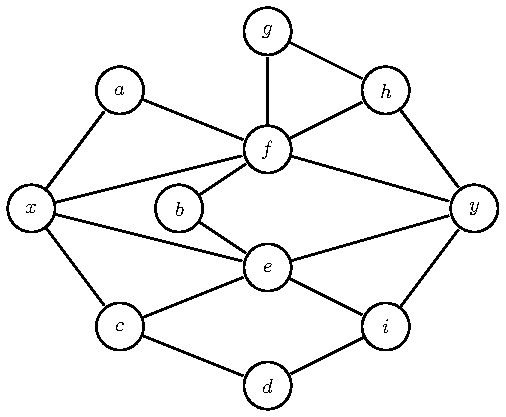
\includegraphics[scale=.9]{6_1.pdf}
\end{center}
\begin{enumerate}
\item Determine $\kappa(x,y)$ and give an example of an $x,y$-cut of size $\kappa(x,y)$.\m
The set $\{f,e,d\}$ is a $x,y$-cut of size 3. There are also 3 disjoint paths from $x$ to $y$, namely: $x,f,y$; $x,e,y$; $x,c,d,i,y$. Since there are 3 for both, we know by Mengar's theorem that $\kappa(x,y) = 3$.
\item Determine $\kappa'(x,y)$ and give an example of an $x,y$-disconnecting set of size $\kappa'(x,y)$.\m
The set $\{xa,xf,xe,xc\}$ is a disconnecting set of size 4. There are 4 edge disjoint $x,y$-paths, namely: $xa,af,fg,gh,hy$; $xf,fy$; $xe,ey$; $xc,cd,di,iy$. So by a theorem that is similar to Mengar's theorem which is inappropriately named Mengar's II theorem (I think it should be named Mengar's$'$ Theorem because the functions are primed), we know that $\kappa'(x,y) = 4$.
\end{enumerate}

\end{enumerate}
\end{document}
